\documentclass[11pt,a4paper]{article}

% ---------- Packages ----------
\usepackage[T1]{fontenc}
\usepackage[utf8]{inputenc}
\usepackage{lmodern}
\usepackage{microtype}
\usepackage{graphicx}
\usepackage{amsmath,amssymb}
\usepackage{booktabs}
\usepackage[margin=1in]{geometry}
\usepackage{float}
\usepackage{xcolor}
\usepackage{enumitem}
\usepackage{titlesec}
\usepackage{caption}
\usepackage{fancyhdr}
\usepackage[hidelinks]{hyperref}

% ---------- Visual style ----------
\definecolor{accent}{HTML}{243B53}
\definecolor{muted}{HTML}{52606D}

\titleformat{\section}
  {\Large\bfseries\color{accent}}
  {\thesection}{0.7em}{}
\titleformat{\subsection}
  {\large\bfseries\color{muted}}
  {\thesubsection}{0.6em}{}

\captionsetup{
  font=small,
  labelfont=bf,
  justification=centering
}

\setlist[itemize]{leftmargin=1.5em}
\setlength{\parindent}{0pt}
\setlength{\parskip}{0.65em}

\pagestyle{fancy}
\fancyhf{}
\fancyhead[L]{DeepIctal-Bonn}
\fancyhead[R]{EEG Seizure Detection}
\fancyfoot[C]{\thepage}
\renewcommand{\headrulewidth}{0.4pt}

\hypersetup{
  colorlinks=true,
  linkcolor=accent,
  citecolor=accent,
  urlcolor=accent
}


% ---------- Document ----------
\title{\textbf{DeepIctal-Bonn}\\[0.4em]
	\large An LSTM-Based Pipeline for Automated Epileptic Seizure Detection from Single-Channel EEG}

\author{
	\textbf{Ali Taghizadeh}\\[0.35em]
	Faculty of Computer Science\\
	Amirkabir University of Technology\\[0.5em]
	\small
	\href{https://github.com/alitkbbl/DeepIctal-Bonn}
	{\texttt{GitHub: github.com/alitkbbl/DeepIctal-Bonn}}
}

\date{\today}

\begin{document}
	
	\maketitle
	\vspace{-1em}



\begin{abstract}
Epileptic seizures can be difficult to identify reliably from long EEG recordings, and manual review is both time-consuming and dependent on expert interpretation. This report describes \textbf{DeepIctal-Bonn}, an end-to-end deep learning pipeline for binary seizure detection using the benchmark Bonn University EEG dataset.

The approach keeps the original single-channel signal but reorganizes each recording into short windows before passing it to a compact stacked Long Short-Term Memory (LSTM) network. To make the evaluation reliable, recordings are split by their original identity so that closely related crops cannot appear in different partitions. The pipeline also uses class-weighted training to account for the 4:1 class imbalance and selects the final decision threshold on the validation set with recall as an explicit constraint.

On the held-out test set, the resulting model achieves 97.00\% accuracy, 91.67\% recall, and a ROC-AUC of 0.9977. These results suggest that a relatively small LSTM can distinguish ictal from non-ictal activity effectively on this benchmark when the data preparation and evaluation procedure are designed carefully.
\end{abstract}

\newpage
\tableofcontents
\newpage

\section{Introduction}

Electroencephalography (EEG) provides a direct view of the brain's electrical activity and remains an important tool in the assessment of epilepsy. Reviewing EEG recordings manually, however, can take considerable time and requires experienced interpretation. This has motivated the development of automated methods that can flag seizure activity for further clinical review.

The Bonn University EEG dataset~\cite{andrzejak2001} is a commonly used benchmark for this type of problem. It contains five groups of single-channel EEG recordings, denoted Z, O, N, F, and S. Each group contains 100 recordings, covering healthy activity as well as seizure-free and ictal recordings.

In this project, the task is reduced to a binary classification problem: distinguishing \textit{ictal (seizure)} recordings from a combined \textit{normal/interictal} class. Rather than engineering a large set of handcrafted features, the model learns temporal representations directly from windowed versions of the raw EEG signal.

\section{Data Preparation}

\subsection{Dataset and Class Definition}

The Bonn dataset contains 500 recordings, with 100 recordings in each of the five sets. Each recording consists of 4097 samples collected at 173.61 Hz, corresponding to approximately 23.6 seconds of EEG.

For this study, the original groups are mapped into two classes:

\begin{table}[H]
\centering
\begin{tabular}{@{}llc@{}}
\toprule
\textbf{Class} & \textbf{Bonn set(s)} & \textbf{Label} \\
\midrule
Ictal / Seizure & S & 1 \\
Normal / Interictal & Z, O, N, F & 0 \\
\bottomrule
\end{tabular}
\caption{Mapping of the five Bonn EEG sets to the two classification labels.}
\end{table}

This produces 100 positive recordings and 400 negative recordings, giving an approximately 4:1 class imbalance.

\subsection{Windowing the EEG Signal}

A raw recording contains 4097 samples. Feeding the entire sequence directly into an LSTM would require the recurrent network to process 4097 time steps, which is unnecessarily long for this dataset and can make optimization more difficult.

Instead, each recording is reorganized into 23 time steps, with 178 samples treated as the feature vector at each step:

\begin{equation}
\mathbf{x} \in \mathbb{R}^{4097}
\longrightarrow
\mathbf{X} \in \mathbb{R}^{23 \times 178},
\qquad
23 \times 178 = 4094.
\end{equation}

Each step therefore represents roughly 1.03 seconds of signal. The LSTM processes 23 recurrent steps rather than 4097 individual samples, reducing the effective sequence length by a factor of about 178 while still retaining the local structure of the original waveform.

\subsection{Micro-Shift Augmentation}

The reshaped representation uses 4094 of the 4097 available samples, leaving three samples unused. Rather than discarding this small portion of the recording, four closely overlapping crops are generated using offsets from 0 through 3:

\begin{equation}
\mathbf{X}^{(o)}
=
\operatorname{reshape}
\left(
\mathbf{x}[o:o+4094],
(23,178)
\right).
\end{equation}

This produces four samples from each original recording and increases the dataset from 500 to 2000 training examples without requiring any additional labels. Importantly, the class proportions remain unchanged.

\subsection{Leakage-Safe Data Splitting}

Because the four crops from a single recording differ by only a few samples, they are highly correlated. A conventional random split at the crop level could therefore place near-duplicate signals in both the training and test sets, leading to overly optimistic performance estimates.

To avoid this, the split is performed using the parent recording as the grouping variable. \texttt{GroupShuffleSplit} keeps all four crops from a given recording in the same partition.

\begin{table}[H]
\centering
\begin{tabular}{@{}lc@{}}
\toprule
\textbf{Split} & \textbf{Samples} \\
\midrule
Train & 1400 \\
Validation & 300 \\
Test & 300 \\
\bottomrule
\end{tabular}
\caption{Grouped train, validation, and test split sizes.}
\end{table}

The resulting partition corresponds to a 70/15/15 split at the recording level.

\subsection{Feature Scaling}

Feature scaling is performed without using information from the held-out partitions. A \texttt{StandardScaler} is fitted only on the training data, after flattening the time-step dimension to obtain an array of shape $(N_{\mathrm{train}}\times T,F)$. The fitted scaler is then applied to the training, validation, and test tensors.

This procedure keeps the normalization step independent of the validation and test statistics.

\section{Model Architecture}

The classifier is a compact stacked LSTM implemented in TensorFlow/Keras. The architecture is intentionally modest, reflecting the relatively small size of the dataset.

\begin{table}[H]
\centering
\begin{tabular}{@{}lll@{}}
\toprule
\textbf{Layer} & \textbf{Configuration} & \textbf{Role} \\
\midrule
LSTM & 64 units, return sequences, L2=$10^{-4}$ & Temporal feature extraction \\
Batch Normalization & --- & Activation stabilization \\
Dropout & 0.35 & Regularization \\
LSTM & 32 units, L2=$10^{-4}$ & Sequence summarization \\
Batch Normalization & --- & Activation stabilization \\
Dropout & 0.35 & Regularization \\
Dense & 16 units, ReLU & Non-linear projection \\
Dropout & 0.20 & Regularization \\
Dense & 1 unit, sigmoid & Seizure probability \\
\bottomrule
\end{tabular}
\caption{DeepIctal-Bonn LSTM architecture. The model contains 75,553 trainable parameters.}
\end{table}

The network is trained with Adam using an initial learning rate of $10^{-3}$, together with binary cross-entropy loss. Because the negative class is four times larger than the positive class, class weights of $w_0=0.627$ and $w_1=2.465$ are used during training. These weights follow the standard balanced-class heuristic

\begin{equation}
w_c = \frac{N}{K\cdot N_c}.
\end{equation}

Early stopping is also enabled with a patience of 15 epochs. When training stops, the weights associated with the lowest validation loss are restored.

\subsection{Choosing the Decision Threshold}

The default sigmoid threshold of 0.5 is not necessarily the most appropriate operating point for seizure detection. In this setting, missing a seizure can be more consequential than generating an additional false alarm, so recall is treated as an explicit requirement.

The threshold is selected using the validation set by maximizing precision while requiring recall to remain at or above 0.90:

\begin{equation}
\tau^*
=
\operatorname*{arg\,max}_{\tau:\,
\mathrm{Recall}_{val}(\tau)\geq0.9}
\mathrm{Precision}_{val}(\tau).
\end{equation}

Once selected, the threshold is fixed and used unchanged on the test set. This keeps the test set independent of the threshold-selection process.

\section{Results}

\subsection{Training Dynamics}

Training stopped after 27 epochs following a plateau in validation loss. The best validation loss was 0.0556.

\begin{figure}[H]
\centering
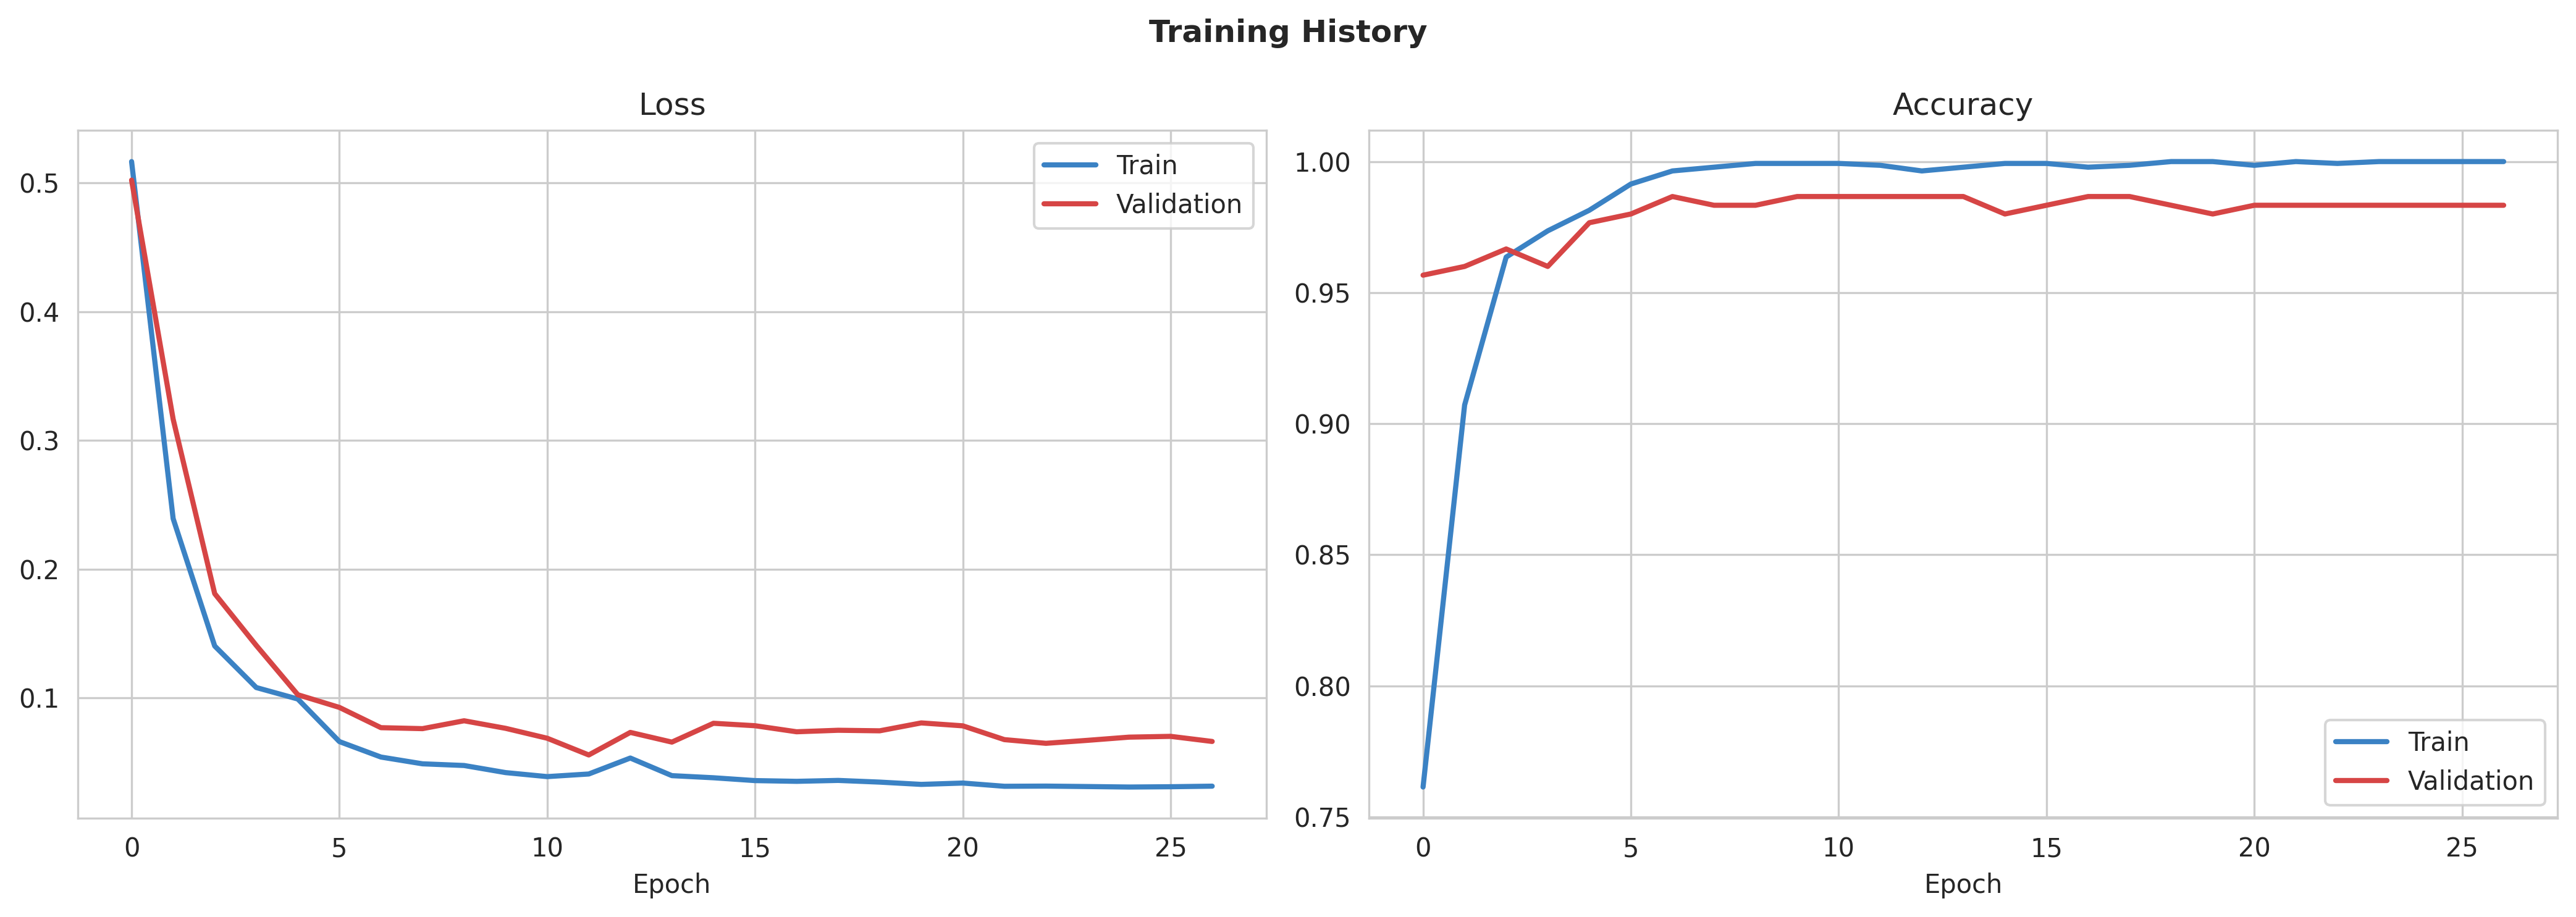
\includegraphics[width=0.95\textwidth]{../figures/training_curves.png}
\caption{Training and validation loss and accuracy over the training process.}
\label{fig:training}
\end{figure}

\subsection{Validation-Based Threshold Selection}

The validation precision--recall curve was used to select the final operating threshold. The resulting threshold was $\tau=0.913$.

\begin{figure}[H]
\centering
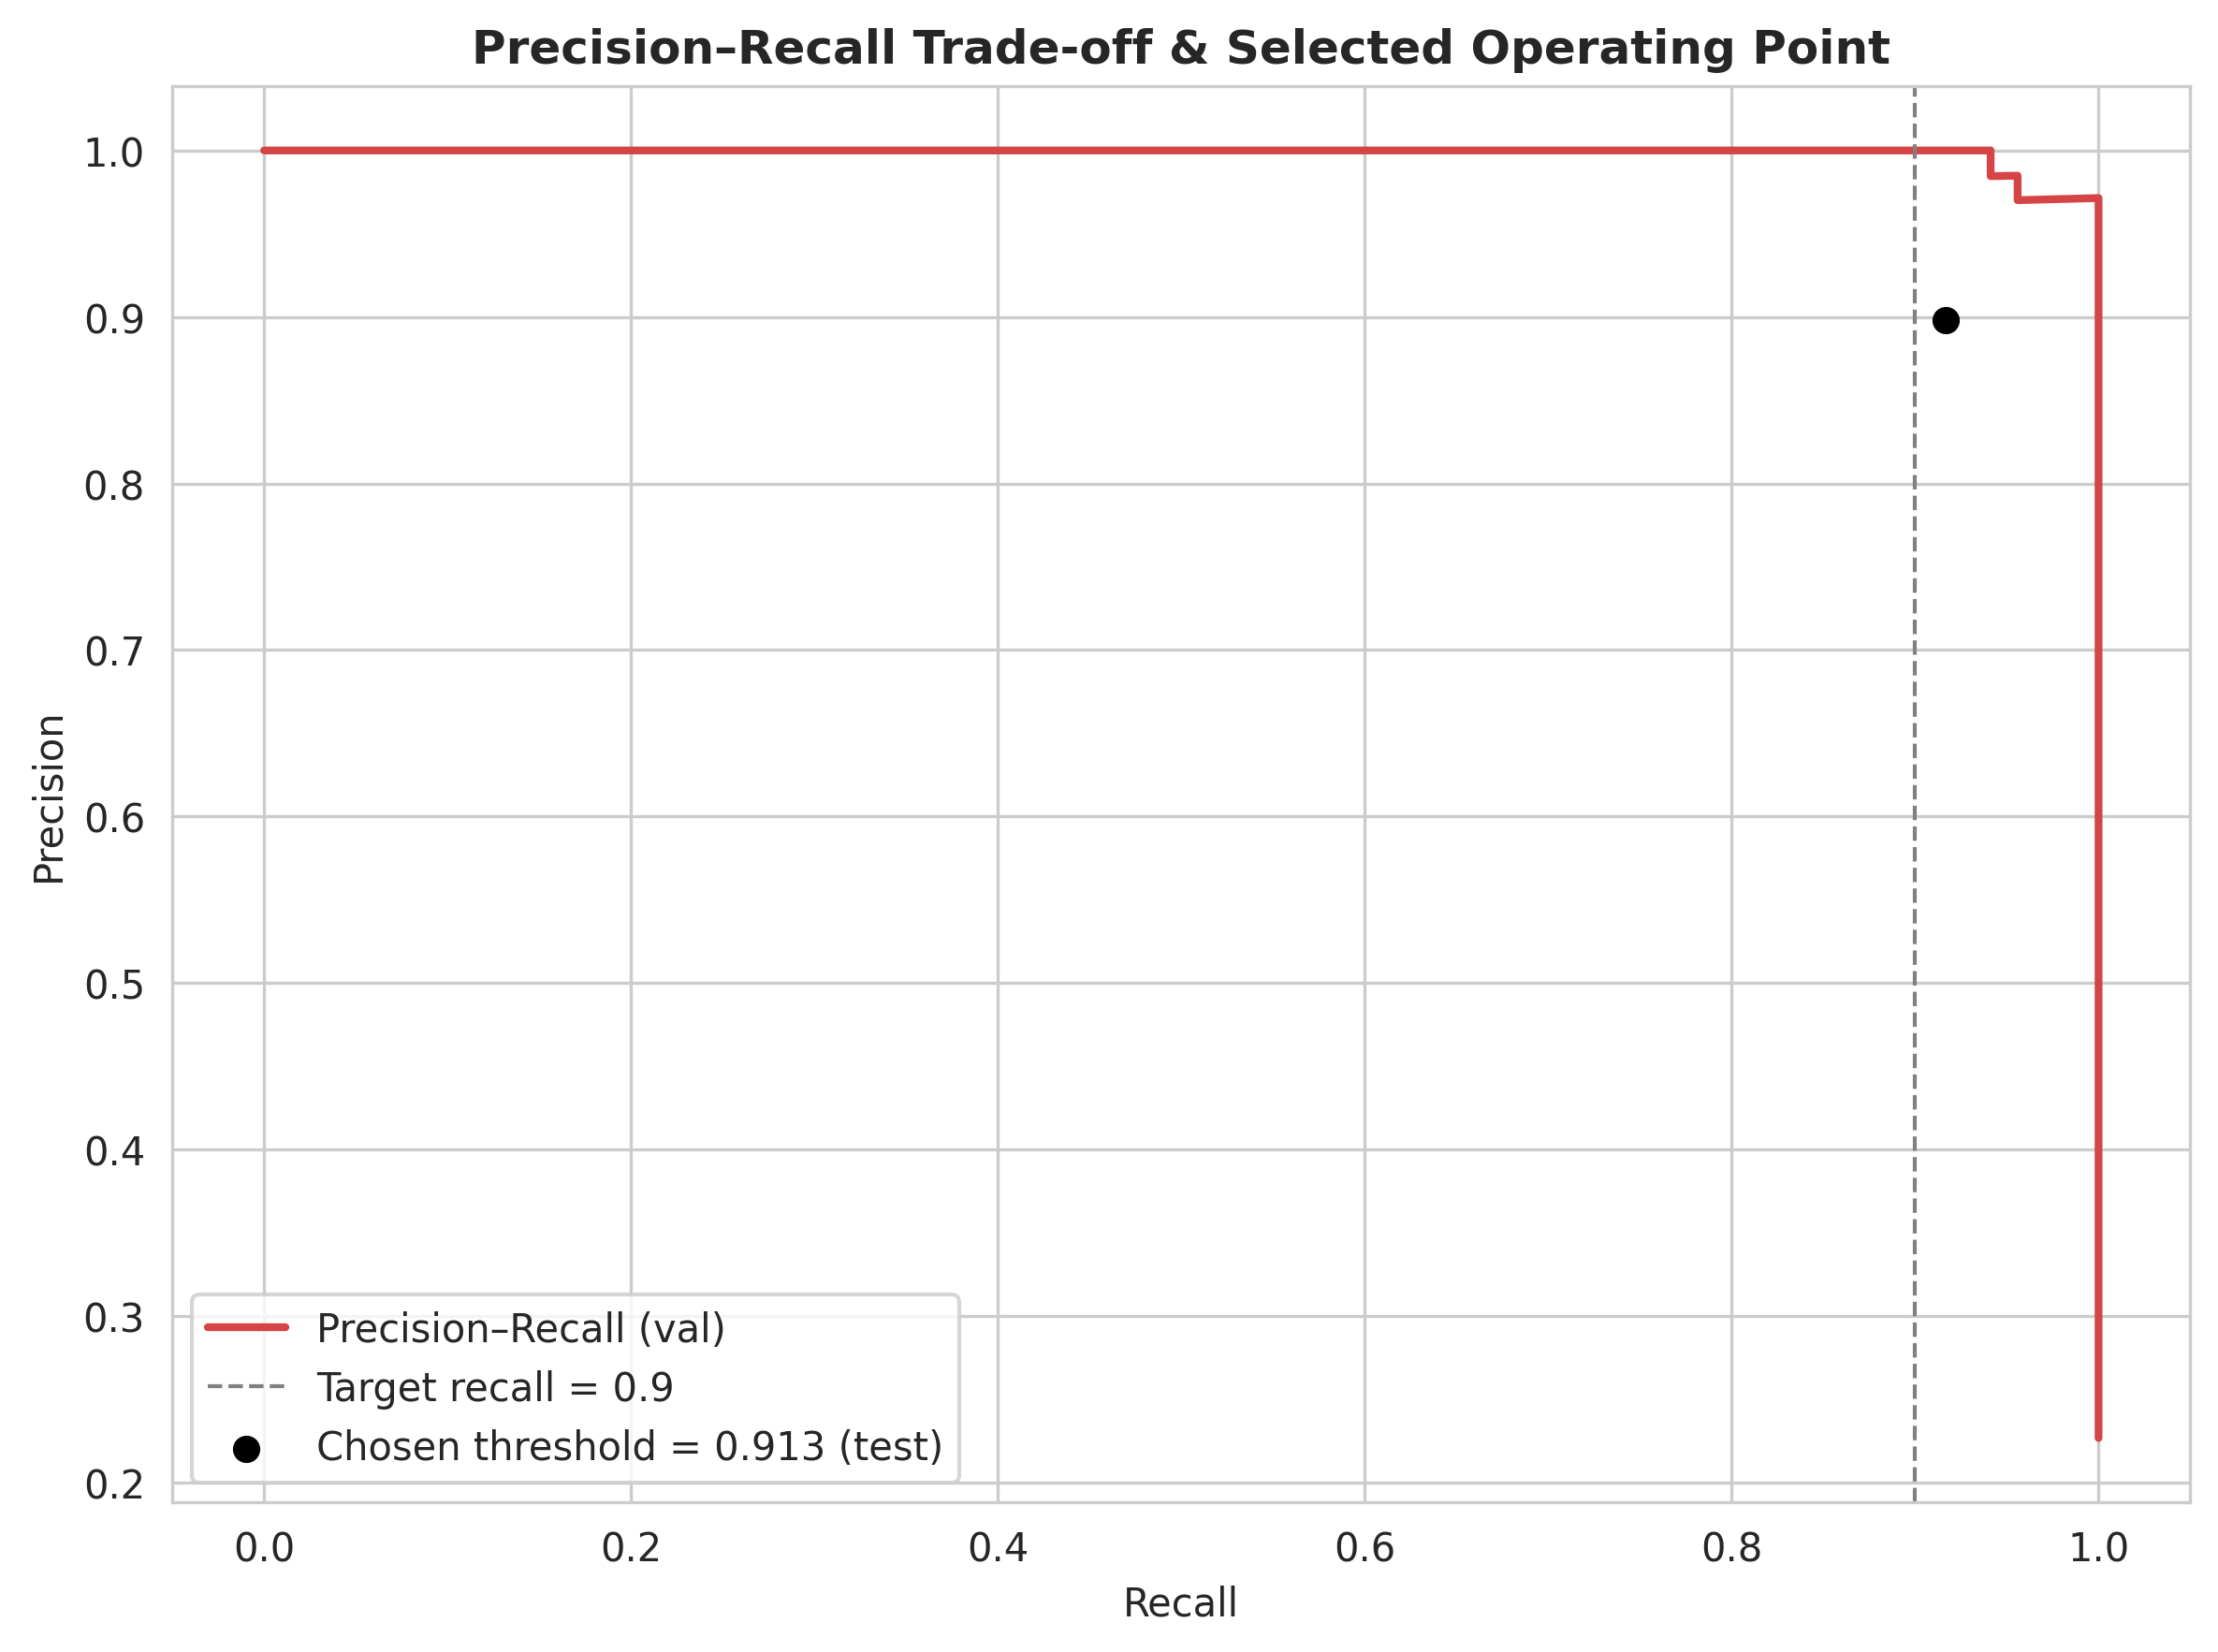
\includegraphics[width=0.7\textwidth]{../figures/precision_recall_curve.png}
\caption{Validation precision--recall curve and the selected operating point.}
\label{fig:pr}
\end{figure}

\subsection{Test-Set Performance}

The final evaluation compares the recall-oriented threshold with the conventional 0.5 threshold.

\begin{table}[H]
\centering
\begin{tabular}{@{}lcc@{}}
\toprule
\textbf{Metric} & \textbf{Tuned ($\tau=0.913$)} & \textbf{Default ($\tau=0.5$)} \\
\midrule
Accuracy & 97.00\% & 97.00\% \\
Precision & 89.80\% & 88.24\% \\
Recall (Sensitivity) & \textbf{91.67\%} & 93.75\% \\
F1-Score & 90.72\% & 90.91\% \\
ROC-AUC & \multicolumn{2}{c}{0.9977} \\
\bottomrule
\end{tabular}
\caption{Test-set performance at the tuned and default decision thresholds.}
\label{tab:metrics}
\end{table}

At the tuned threshold, the confusion matrix contains 247 true negatives, 5 false positives, 4 false negatives, and 44 true positives.

\begin{figure}[H]
\centering
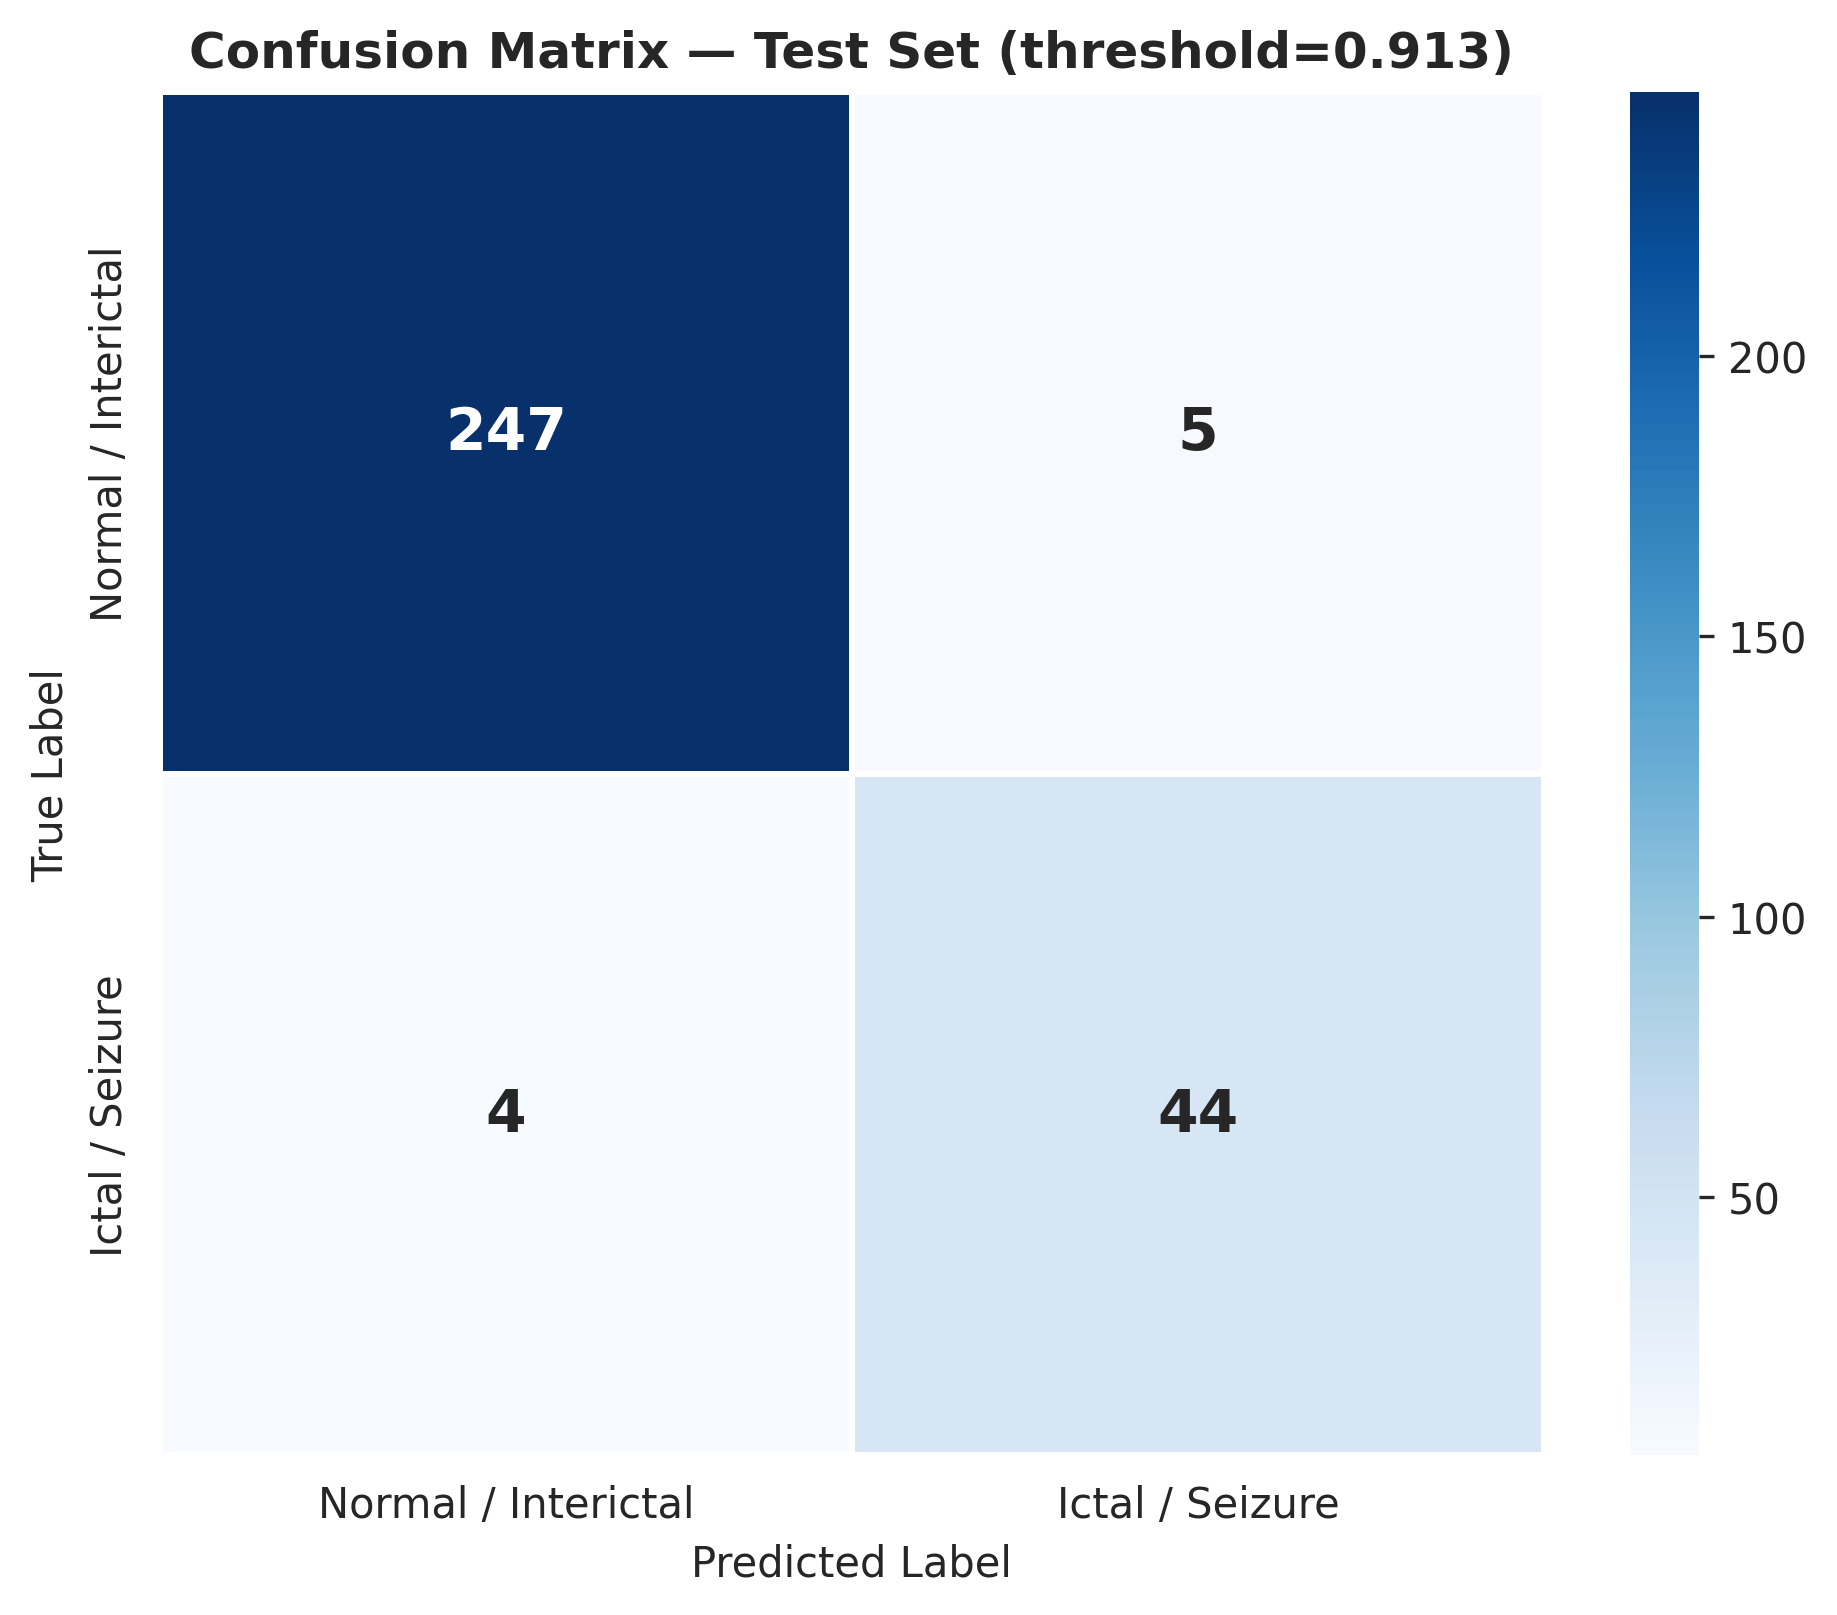
\includegraphics[width=0.6\textwidth]{../figures/confusion_matrix.png}
\caption{Confusion matrix on the held-out test set at $\tau=0.913$.}
\label{fig:cm}
\end{figure}

\begin{figure}[H]
\centering
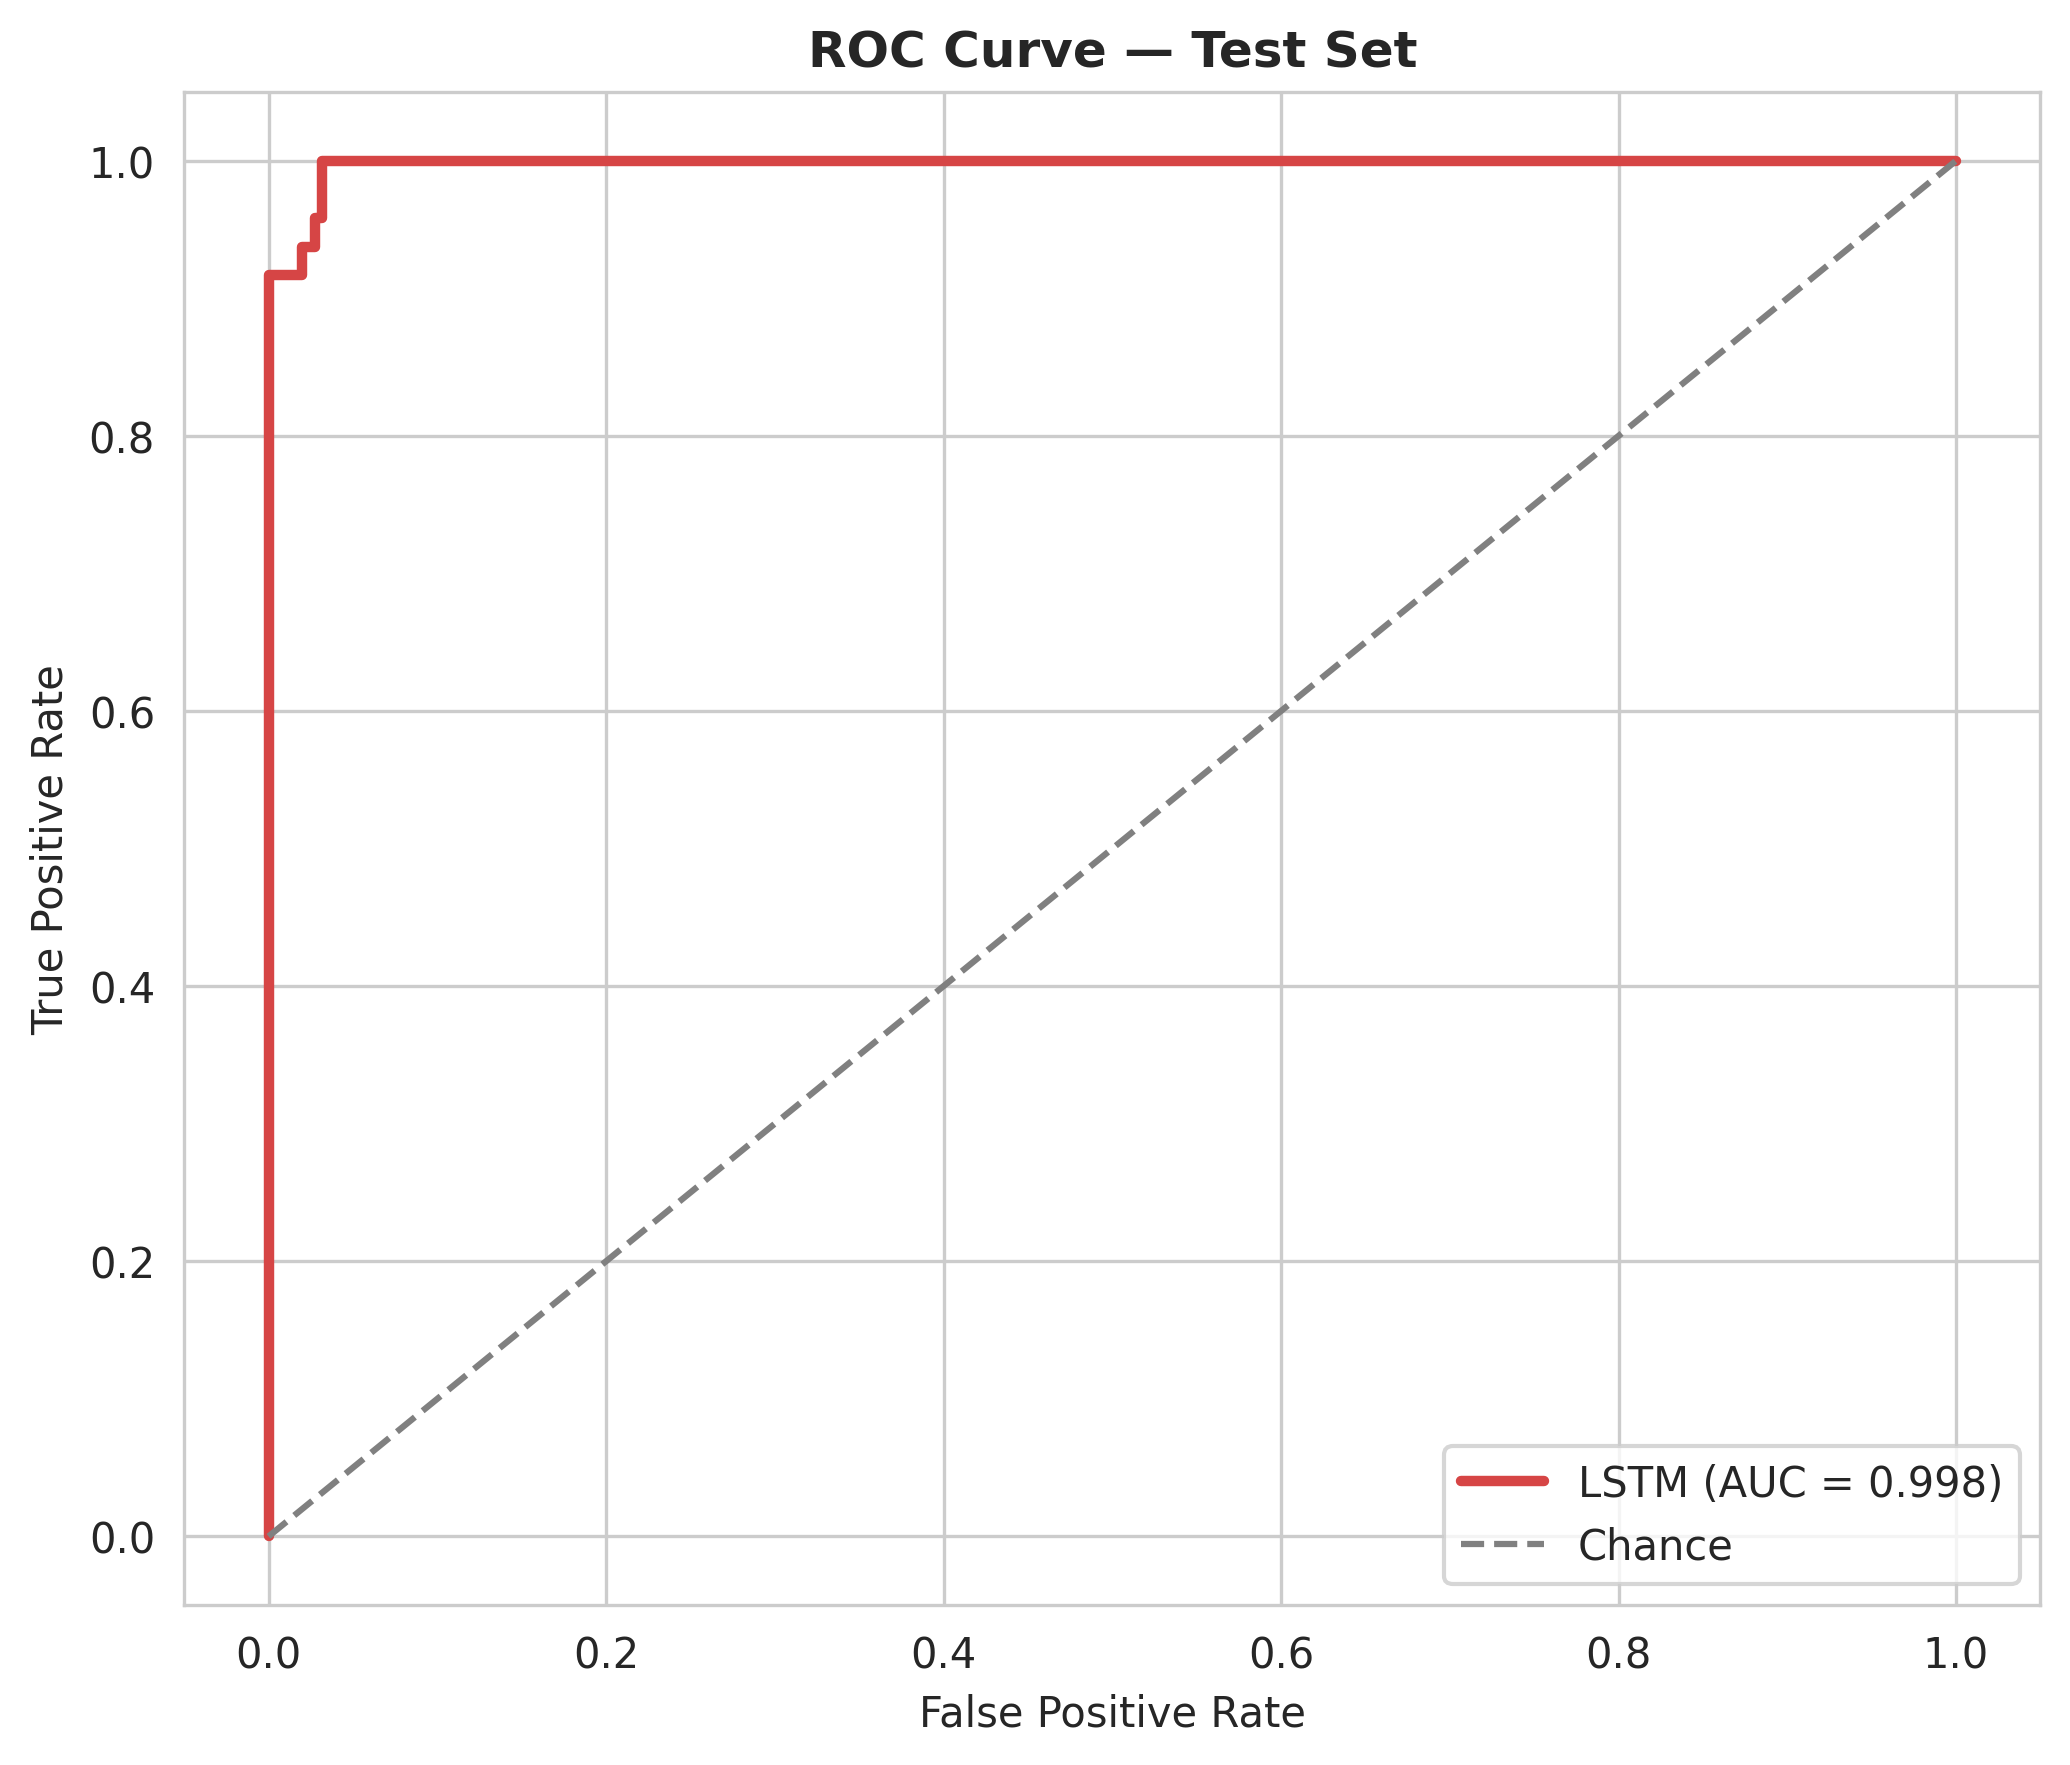
\includegraphics[width=0.65\textwidth]{../figures/roc_curve.png}
\caption{Receiver Operating Characteristic curve (ROC-AUC = 0.9977).}
\label{fig:roc}
\end{figure}

\subsection{Exploratory Signal Analysis}

The raw EEG signals also show visible differences between the two classes. In the representative time-domain traces, ictal activity generally has larger amplitudes and a more pronounced oscillatory structure than the normal/interictal examples.

\begin{figure}[H]
\centering
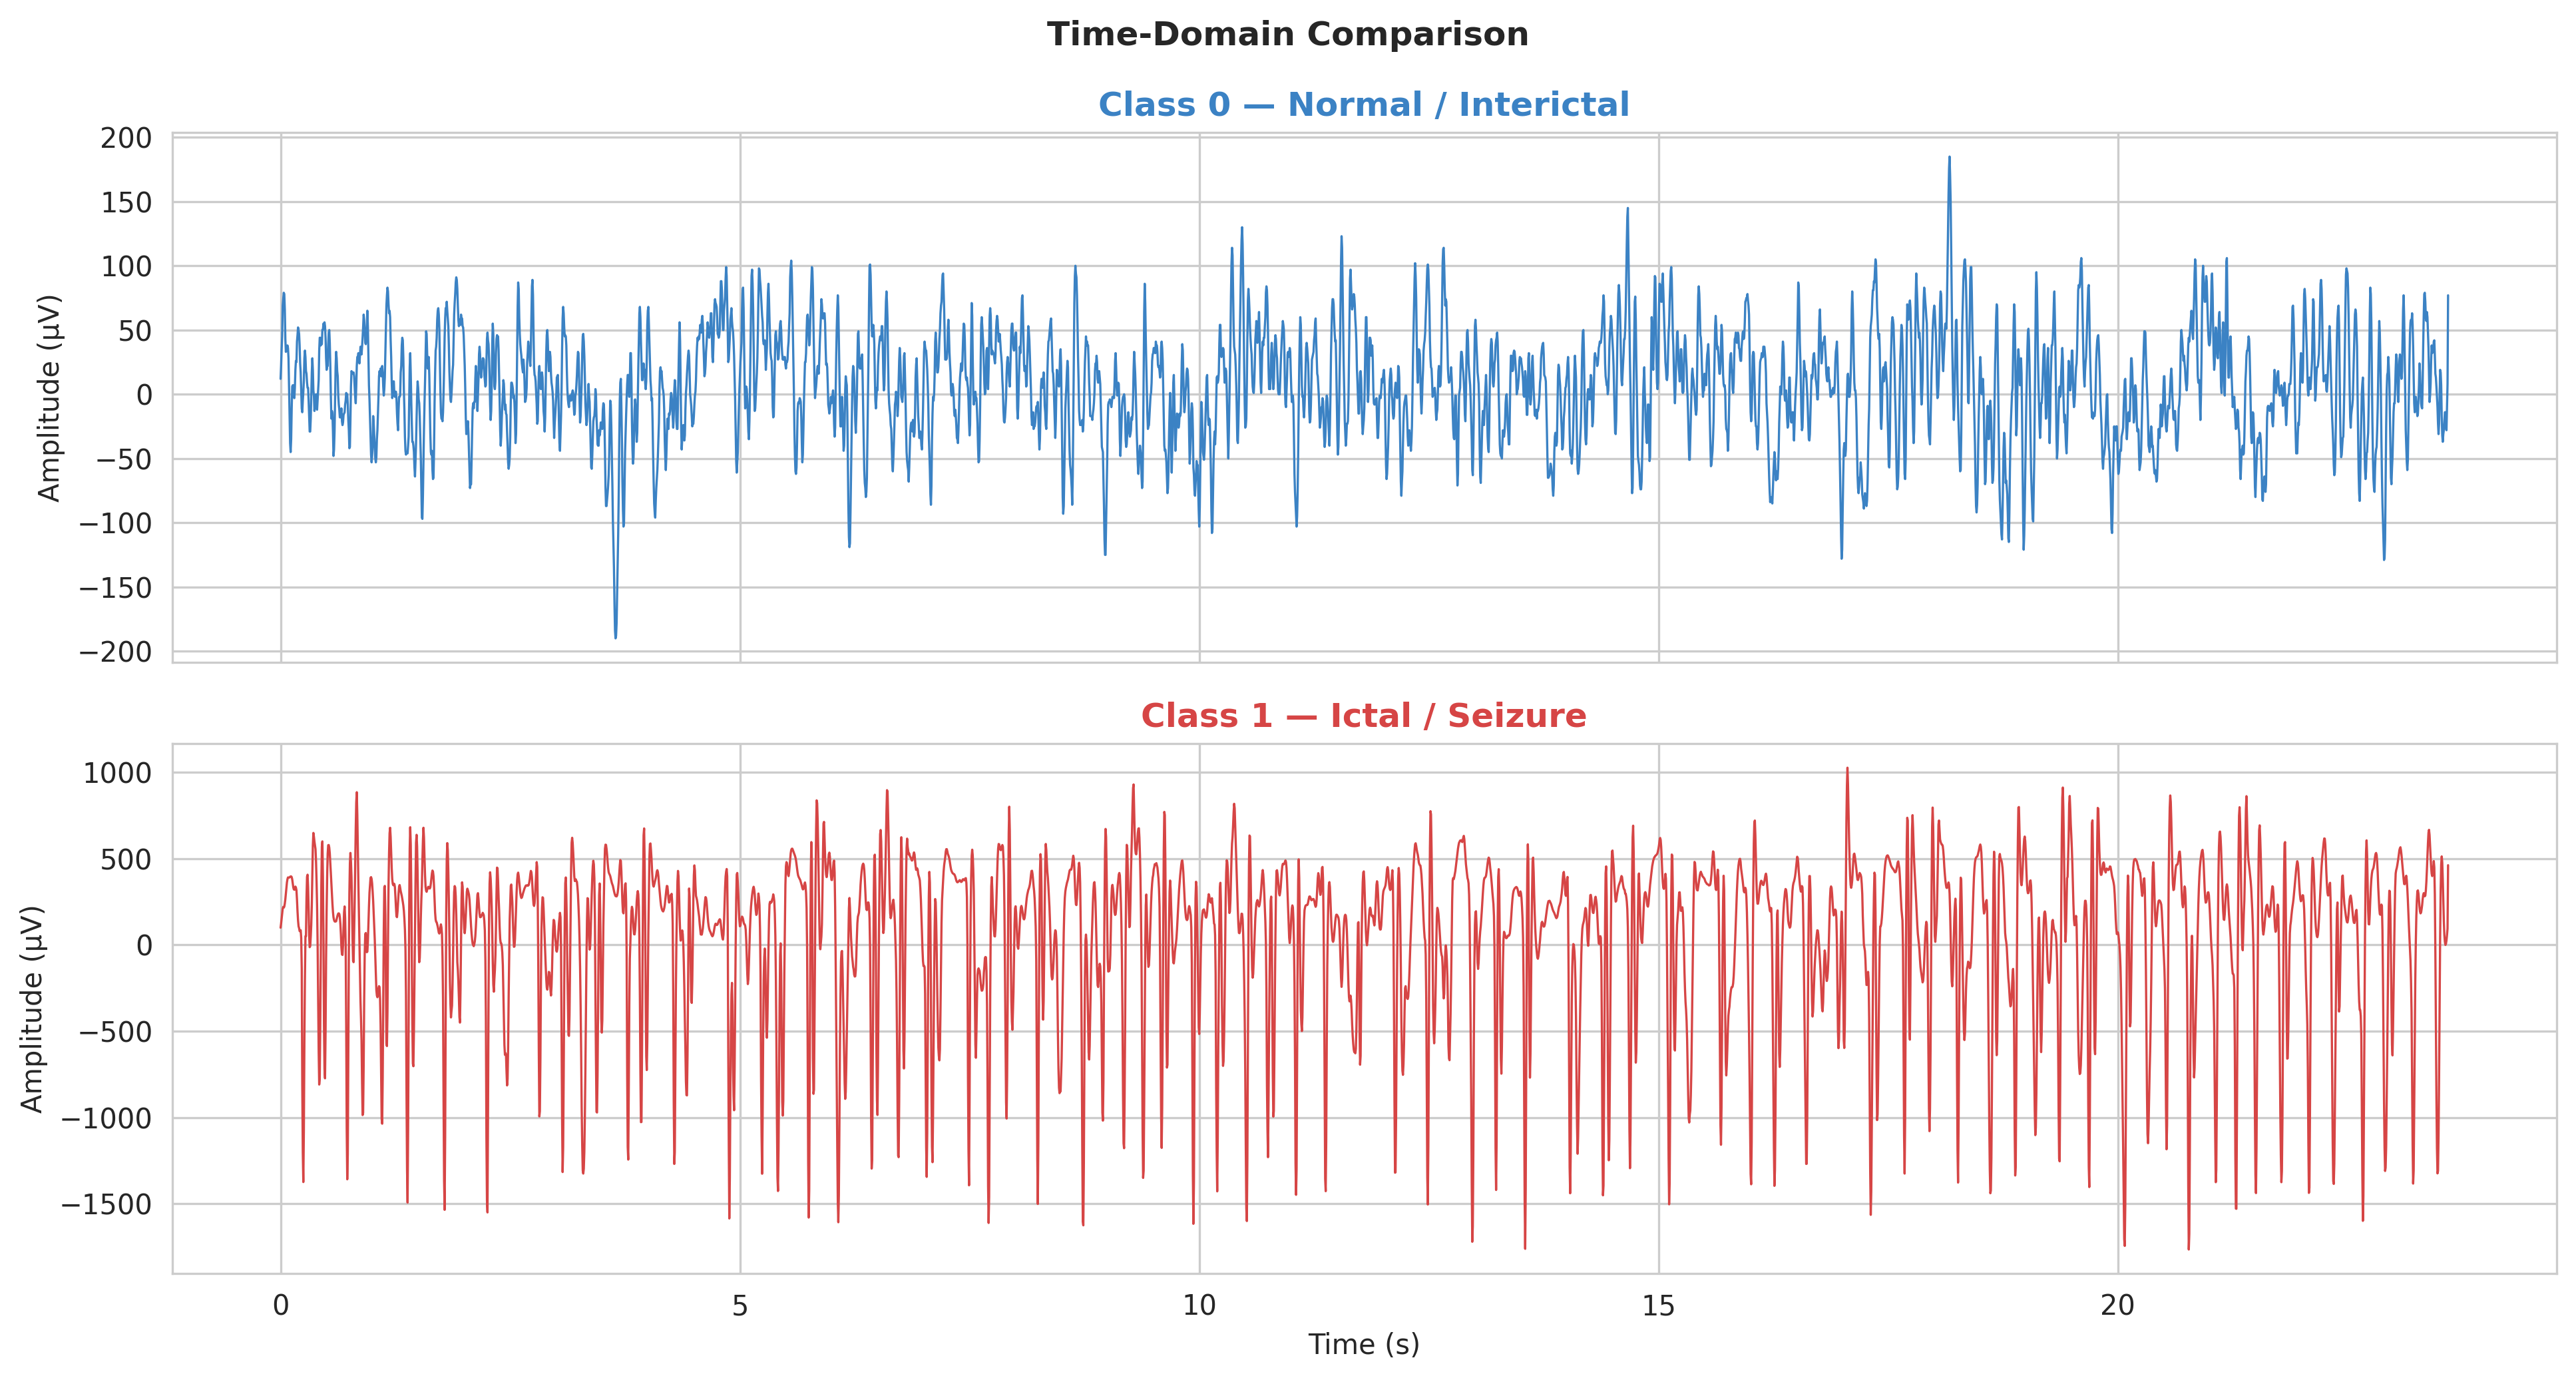
\includegraphics[width=0.95\textwidth]{../figures/time_domain_comparison.png}
\caption{Representative time-domain EEG traces for normal/interictal and ictal activity.}
\label{fig:timedomain}
\end{figure}

The power spectral density analysis provides a complementary view. On average, the ictal recordings show stronger low-frequency spectral power than the normal/interictal recordings.

\begin{figure}[H]
\centering
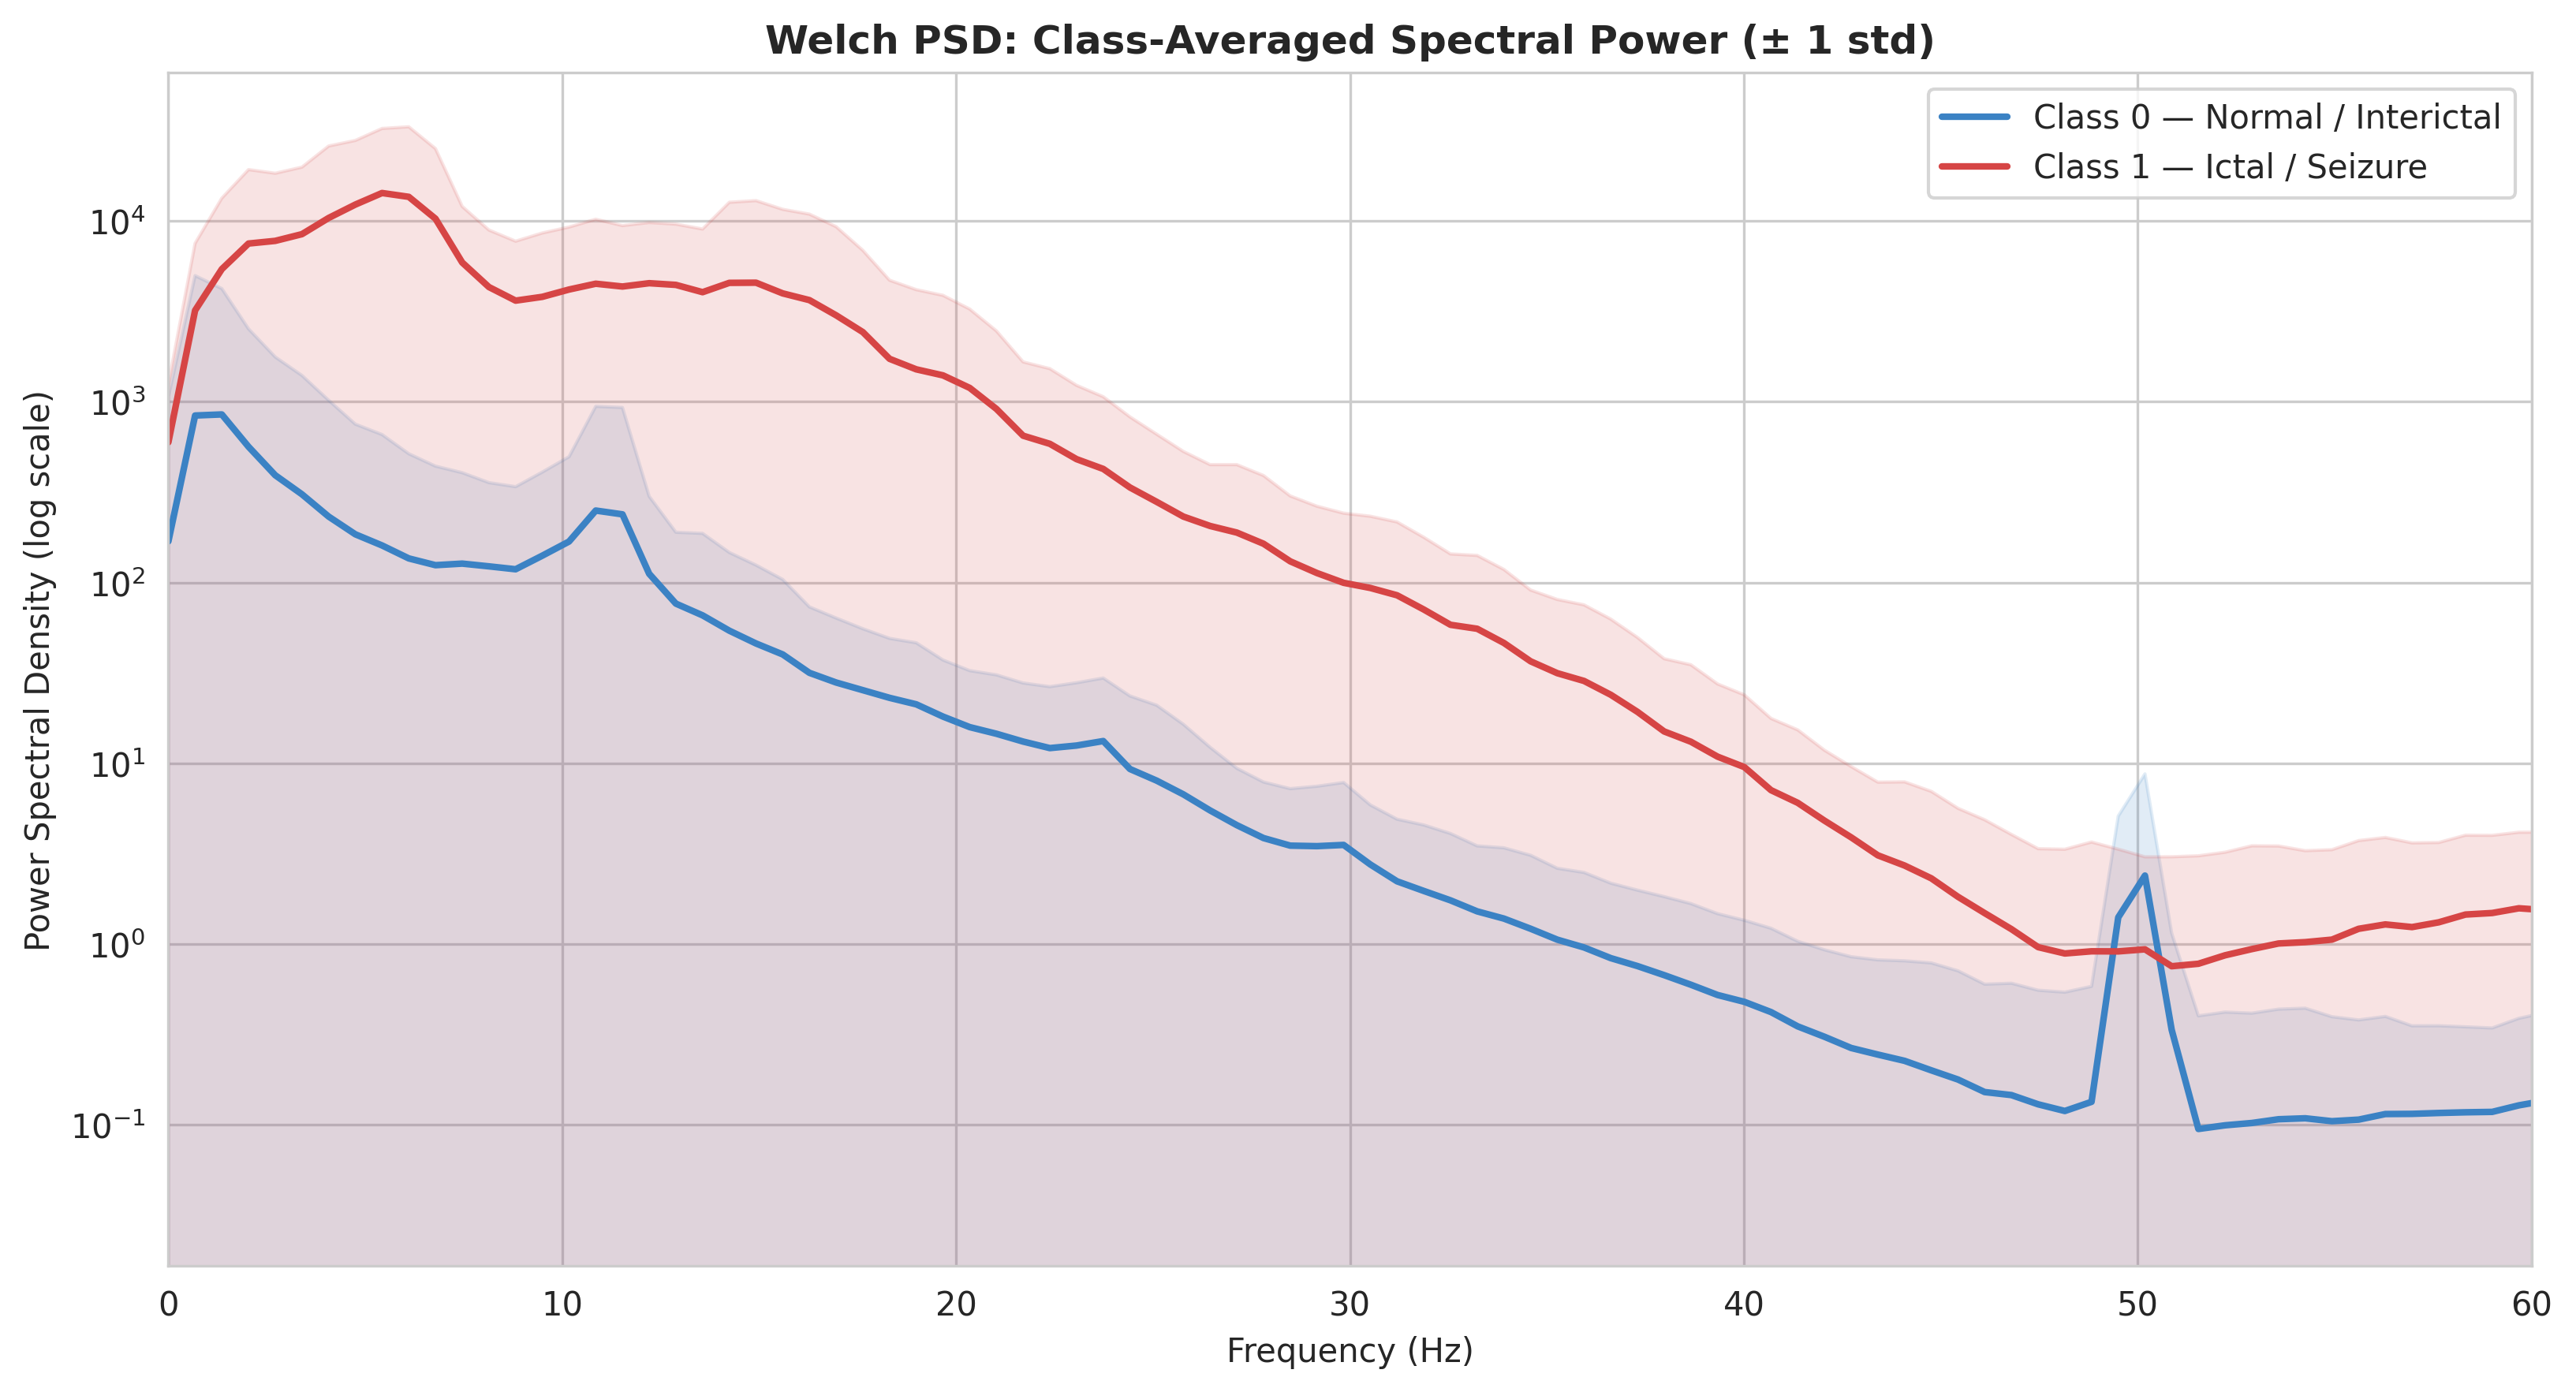
\includegraphics[width=0.75\textwidth]{../figures/psd_comparison.png}
\caption{Class-averaged Welch power spectral density; the shaded region represents $\pm1$ standard deviation.}
\label{fig:psd}
\end{figure}

\section{Discussion}

The results show that the proposed windowed LSTM can separate ictal from non-ictal EEG activity effectively on the Bonn benchmark, even when only a single EEG channel is available. The strong ROC-AUC of 0.9977 indicates that the model ranks the two classes very well across operating thresholds.

A particularly important part of the pipeline is the way the augmented samples are split. The four micro-shifted crops from each recording are almost identical, so treating them as independent observations during the split would allow information from the same underlying recording to appear in multiple partitions. Grouped splitting prevents this and gives a more credible estimate of generalization.

Class weighting is also important because the dataset contains four times as many negative recordings as positive recordings. Without compensation, the model could obtain a deceptively strong accuracy by favoring the majority class.

The threshold analysis illustrates another practical point. The tuned threshold of 0.913 slightly improves precision while maintaining recall above 90\%, although the default threshold actually gives marginally higher recall and F1 on this particular test set. The main value of threshold selection is therefore methodological: it defines the operating point using the validation data rather than choosing 0.5 arbitrarily or tuning directly on the test set.

These results should nevertheless be interpreted in the context of the Bonn benchmark. Its recordings are relatively small and controlled compared with heterogeneous clinical EEG collected in real-world settings. High benchmark performance does not, by itself, establish clinical readiness.

\section{Conclusion}

This report presented DeepIctal-Bonn, a compact and reproducible LSTM pipeline for binary seizure detection from single-channel EEG. The main design choices were motivated by the structure of the data: short windowed sequences make recurrent processing more manageable, micro-shift augmentation increases the number of training examples, grouped splitting prevents near-duplicate leakage, and class weighting compensates for the imbalanced labels.

Using these components together, the model achieved 97.00\% accuracy, 91.67\% recall, and a ROC-AUC of 0.9977 on the held-out test set.

There are several natural directions for extending the work. A next step would be to evaluate the approach on larger and more heterogeneous clinical datasets, where the model would face greater variation between subjects and recording conditions. It would also be useful to investigate multi-channel EEG and alternative sequence models, including transformer-based architectures.

\begin{thebibliography}{9}

\bibitem{andrzejak2001}
Andrzejak, R. G., Lehnertz, K., Mormann, F., Rieke, C., David, P., \& Elger, C. E. (2001).
Indications of nonlinear deterministic and finite-dimensional structures in time series of
brain electrical activity: Dependence on recording region and brain state.
\textit{Physical Review E}, 64(6), 061907.

\end{thebibliography}

\end{document}
